\section{Planlægning af begivenheder}
Planlægningen af hvilke begivenheder der skal køres hvornår, tager udgangspunkt i det overordnede formål med systemet. Generelt vil formålet være at minimere antallet af overskredne deadlines, men dette er sjældent det eneste kriterie der planlægges efter, ofte vil prioriteten for, og tiden det tager at udføre en begivenhed indgå i planlægningen. Eksempelvis vil man ofte prioritere at nå en kritisk deadline selv om det betyder at man overskrider to soft deadlines. 

%De fleste eksisterende real-time systemer arbejder på isolerede systemer, hvor planlæggeren har fuld kontrol over hele computeren. Derfor er hovedparten af forskningen indefor området gået til udarbejdelsen af specialiserede kerner og komplette operativsystemer\cite{damm1989real, jones1979staros, levi1989maruti,ramamritham14scheduling}. Vi ønsker i modsætning hertil ikke at udvikle en specialiseret kerne, men lade \sched en i \pycsp kunne planlægge processer efter bedste evne baseret på informationer den har om processerne.

For at foretage en planlægning af begivenheder der opfylder systemets formål bedst muligt, skal vi have så meget information om begivenheder som muligt - jo mere vi ved om dem jo bedre en planlægning kan der foretages. De relevante informationer i forhold til planlægningen er, hvornår en begivenhed forekommer, hvor lang tid den tager at udføre samt hvilken prioritet den har. 

Ud fra den tilgængelige viden kan der foretages en statisk eller dynamisk planlægning\cite{cheng1987scheduling}. Statisk RTP kræver at vi har alle de nævnte informationer om alle begivenheder. Herved kan vi på forhånd foretage en fuldstændig planlægning og allerede inden start have klarlagt om nogen deadlines vil blive overskredet. Såfremt vi ikke har alle informationer til rådighed, er vi nødsaget til at foretage en dynamisk planlægning. Dette vil ofte skyldes at vi enten ikke ved hvornår en begivenhed forekommer, eller at vi ikke har information om hvor lang tid der tager at udføre en begivenhed. I praksis vil det være svært at opstille eksakte værdier for hvor længe en begivenhed er om at blive udført og der benyttes derfor ofte estimater i stedet for. \fxnote{hvilken betydning har det at der benyttes estimater i stedet for eksakte værdier?}

%Overordnet kan begivenheder planlægges enten statisk eller dynamisk\cite{cheng1987scheduling}. I statisk RTP er alle begivenheder kendt på forhånd. Planlæggeren kan i dette tilfælde allerede inden start udregne om det er muligt at overholde alle deadlines. Alternativt planlægges begivenhederne dynamisk hvis der uregelmæssigt kan ankomme nye begivenheder der skal planlægges. 

%\fxnote{Motivationen her skal være at vi skal kende begivenheders frekvens og længde - skriv noget om det!}
%I realtidssystemer er næsten alle begivenheder cykliske, med enten en regelmæssig eller tilfældig frekvens. Begivenheder der forekommer med en regelmæssig frekevens kan være f.eks. være målinger der skal foretages med bestemte intervaller, hvor uregelmæssig frekvens ofte vil være tilfældet ved begivenheder der skal indtræffe som reaktion på udefrakommende input, f.eks. fejl eller alarmer. 

%\begin{shaded}
%Til planlægningen har planlæggeren behov for at vide hvor lang tid det vil tage at udføre en given begivenhed per periode, men da dette tal enten ikke er kendt eller fast for hver periode, bruges der ofte estimater. Dette medfører at en aperiodisk begivenhed kan ankomme på et vilkårligt tidspunkt og da planlæggeren kun har et estimat for tidsforbruget kan man  ikke tilknytte en ``hard deadline'' til aperiodiske begivenheder, da der altid findes en kæde af aperiodiske begivenheder der medfører en overskridelse af en deadline. 
%\end{shaded}

%\fxnote*{Dette skal måske flyttes eller omformuleres så vi ikke med det samme begrænses til dynamiske \sched}{I \pycsp kan der til alle tidspunkter tilføjes nye processer, og derfor vil vi kun beskæftige os med en dynamisk \sched. Desuden har man ikke med \pycsp fuld kontrol over hele operativsystemet. Mængden af processerkraft vi har til rådighed til kørsel af processerne vil derfor varriere uafhængigt af \pycsp, hvorfor vi heller ikke kan lave et pålidelig ``hard real-time system'', men fokusere på et ``soft real-time system''.}

\subsection{Metoder til skemaplanlægning}
Der findes adskillige metoder til at planlægge rækkefølgen af begivenheder. De adskiller sig fra hinanden med henblik på hvilke informationer der er til rådighed og hvad de optimerer efter. Vi har valgt at kigge på ``Rate monotonic algorithm''\cite{lehoczky1989rate,liu1973scheduling} og ``Earliest deadline first''\cite{liu1973scheduling} indenfor henholdsvis statisk og dynamisk skemaplanlægning.

Hvor processer isoleret set har behov for at udføre deres opgave inden deres deadline, har \sched en behov for kvantitativt at kunne organisere dem indbyrdes, således den til enhver tid kan vælge hvilken proces der skal udføres som den næste. Hovedformålet for en  \sched ~ er derfor at gå fra en række processer med tilknyttet deadline og eventuelt andre egenskaber til en prioriteret liste. \\
Der fokuseres i litteraturen på om en algoritme er stabil eller ej. Såfremt en algoritme er stabil vil man kunne definere en delmægnde af begivenheder, for hvilke man kan garantere at de ikke overskrider deres deadline. 

\subsubsection{Rate monotonic algorithm (RM)}
RM er en statisk \sched, der fra start af udregner en prioriteret liste på baggrund af frekvensen af processens periode, dermed vil processer der oftet skal have udført deres periode en højere prioritet, end processer med lav frekvens. RM er todelt og i første del udføres før selve simuleringen udregnes  prioriteten for processerne, og udvælger hvilke processer der kan medtages i selve udførslen. Anden del står for udvælgelsen af processer  under simuleringen, og her vælges simpelt den proces med den højeste prioritet. 

Et problem for RM er at ved udvælgelsen af processer der kan medtages har man ikke en optimal udnyttelsen af processorkraft. \Citeauthor{lehoczky1989rate} er kommet frem til at ``worst-case'' er udnyttelsen i gennemsnit 88\\cite{lehoczky1989rate}. Et større problem i relation til implementering i \pycsp er dog at RM er dog at den er statisk. Til gengæld er algoritmen stabil ved en overskridelse af deadline for en proces. 

\subsubsection{Earliest deadline first (EDF)}
Som alternativ til den statiske \sched, hvor man ikke kan ændre prioriten af processen løbende under udførslen, findes de dynamiske \sched er, hvor er EDF er et eksempel. Her evalueres prioriterne af processerne dynamisk under udførslen og evaluerer dermed løbende hvilke processer der skal udvælges. I EDF har den proces hvis deadline ligger først højest prioritet og den proces hvis deadline ligger længt ude i fremtiden har lavest prioritet. Aperiodiske processer kan i EDF indgå på lige fod med de periodiske da man til hvert processkift evaluere hvilken der har den nærmeste deadline, som både kan være en periodisk proces som en aperiodisk.

Udnyttelsen af processorkraft kan i EDF komme op på 100\%, da alle processer bliver planlagt løbende i modsætning til RM der foretager et valg om en given proces kan planlægges.  Ulempen ved EDF er den ikke er stabil idet vi ikke har kontrol over hvilke processers deadline der bliver overskredet. Dette er specielt et problem hvis man har en en uhomogen samling processer hvor en mindre del er kritiske. Såfremt skemaplanlæggeren ikke kan foretage preemptive skift mellem begivenheder kan EDF ikke give nogen garanti om at alle deadlines overholdes, selv om der findes en rækkefølge af begivenheder der sikrer dette. Dette er illustreret på \cref{fig:edf-nonpreemptive}.

\begin{figure}
 \begin{center}
  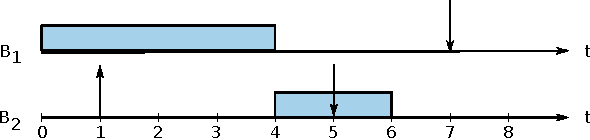
\includegraphics[scale=1.00]{images/edf-nonpreemptive}
  \caption{Overskridelse af deadline med EDF såfremt der ikke kan udføres preemptive kontekstskift. Begivenheden $B_2$ ankommer til tiden $t_1$ og har deadline ved $t_5$. Den kan dog ikke igangsættes før $B_1$ er færdig, hvorved $B_2$ overskrider sin deadline.}
  \label{fig:edf-nonpreemptive}
  \end{center}
\end{figure}



\subsubsection{Least Laxity(LL)}
LL er en modifikation af EDF. LL kigger på hvor lang tid en begivenhed tager at udføre sammenholdt med hvor lang tid der er til deadline for begivenheden. Laxity er defineret som deadline minus tiden det tager at udføre begivenheden. Laxity bliver altså et udtryk for hvor presserende det er at igangsætte en begivenhed for at den kan nå sin deadline. I LL bruges dette til at prioritere de begivenheder der har mindst laxity højest når begivenhederne planlægges. \\
\\
I systemer hvor begivenheder ikke er isolerede men kan have interne afhængigheder, kan der opstå det problem der hedder prioritetsinvertering\cite{sha1990priority}. Dette problem opstår hvis en begivenhed med høj prioritet er afhængig af en begivenhed med en lavere prioritet. Derved bliver begivenheden i praksis kørt med den lavere prioritet da den ikke er klar før begivenheden med lav prioritet er færdig. Problemstillingen kan vises klart med følgende eksempel. Forestil dig tre begivenheder ($B_0,B_1,B_2$)med prioriteterne $Pr_0>Pr_1>Pr_2$. Først udvælges $B_0$ da denne har højst prioritet, men stopper da den er afhængig af kommunikation fra $B_2$. Den næste begivenhed der udvælges vil være $B_1$, og dermed bliver $B_0$ unødigt forsinket mens $B_1$ kører.\\
En ofte benyttet metode til at undgå priotetsinvertering er priotetsnedarvning. Ved at benytte denne løsning vil en begivenhed med lav prioritet, som en begivenhed med høj prioritet er afhængig af, nedarve prioriteten fra den begivenhed der venter på den. Herved sikres det at begivenheder med høj prioritet ikke kommer til at vente unødigt på prioriteter med lav prioritet. \fxnote{flere løsninger på prioritetsinvertering bør nok nævnes.}

